The lunar farside provides a unique accessible environment in that the moon shields it from Earth and near-Earth radio frequency interference at all times.  Therefore, {\em anything} detected is of scientific interest. Since there is no ionospheric blockage, low frequency observations that are impossible from Earth can also be made in an RFI-free environment.  Although the lunar farside will remain an excellent low-RFI site for many years to come, {\em now} is the only time to take completely pristine measurements of the radio spectrum.  This is an opportunity that will never again present itself.

\subsection{Technosignatures}
Humanity's quest to determine its place in the Universe and whether we are its only inhabitants has driven knowledge and imagination since we first looked to the sky.  Many large telescopes are in consideration in order to help determine if other biological processes are happening in nearby stars (called "biosignatures") and we now also have the capability to explore whether technological signatures (technosignatures) exist over a large swath of our Galaxy.  The Breakthrough Listen program has transformed the field and has greatly expanded the search for such technosignatures (e.g. \citealt{Enriquez_2017, Price_2020, Gajjar_2021}.  The greatest impediment is the prevalence of RFI made by essentially every device that is electrically powered.

Signals of interest must be carefully sought within this cacophony of RFI. To differentiate between RFI and a technosignature requires that the technosignature signal is at a frequency/time not inhabited by RFI and the signal must persist and be quite stable over a timeframe of many minutes.  The signals are assumed to be nearly monochromatic and slow-drifting in time.  A series of on-off measurements are used (for single-dish experiments)to make sure that the signal-of-interest is coming from the main beam of the telescope and not RFI in a distant sidelobe.  These techniques are incredibly powerful in conducting senstive searches over the available bandwidth, and have the added benefit being able to use very large earth-based telescopes to dramatically increase the sensitivity.  However, many limitations exist on appropriate ranges of frequency and time, and some frequency ranges are so impacted that searches (and radioastronomy research generally) are infeasible in those bands.  Signals of short duration (a few seconds) or signals heavily modulated are nearly impossible to discern.  And of course, technosignatures ``behind'' RFI is not detectable (or at least believably so).

\subsection{Transients}
The recent flourishing of the field of radio transients (both slow and fast) has brought a wealth of information, significantly advancing various areas of physics. Notably, pulsars and fast radio bursts (FRBs) stand out due to their unique potential to reveal new kinds of physics. These astrophysical phenomena offer valuable insights into gravitational waves, cosmology, and plasma physics, among other fields. However, beamforming radio observations can also shed light on other transients such as flare stars and planetary conditions within and outside the solar system. 

\subsubsection{Pulsars}
Pulsars are highly magnetized, rotating neutron stars that emit beams of electromagnetic radiation. Pulsars serve as precise cosmic clocks, providing insights into the interstellar medium, gravitational waves, and the fundamental physics of matter under extreme conditions. It is theorized that pulsars spin rapidly upon creation and slow down due to gravity over time, along with changes in the medium surrounding the pulsar, which alters the pulse structure as well \citep{LW_2013}. By using coherent beamforming, sensitivity to weak pulses can be improved, and frequency and time resolution can be adjusted to decrease the effects of dispersion measure smearing (e.g. \cite{WL_2020}).\\

Broadband studies of pulsars allow for a study of the emission physics and surrounding material, where the lower frequencies are sensitive to emission closer to the pulsar surface. With ground-based radio telescopes, the ionosphere can create challenges, especially in weaker pulsars that have a peak spectral turn-over between 100--200,MHz \citep{Stappers_2011}. By moving the radio telescope off from the Earth and away from the ionosphere cut-off around 30,MHz, a broader range of pulsar emission physics can be studied than has yet been explored.\\

A farside lunar telescope, shielded from Earth’s radio frequency RFI, would significantly enhance pulsar observations by providing a pristine observational environment. This location allows for low-frequency studies, critical for understanding the early stages of pulsar emission mechanisms and the surrounding interstellar medium. The absence of atmospheric effects enables precise measurements, leading to better constraints on pulsar timing and more accurate tests of general relativity. Furthermore, the lunar farside offers an opportunity to continuously monitor pulsars without the interruptions caused by the Earth’s rotation, increasing the data quality and allowing for the detection of subtle changes in pulsar behavior over time.


\subsubsection{Fast Radio Bursts}
Fast Radio Bursts (FRBs) are intense, millisecond-duration radio pulses originating from extragalactic sources. Their origins remain one of the most intriguing mysteries in modern astrophysics. Although Galactic magnetars have shown to exhibit similar FRB-like emission \cite{BC_2020}, the exact origins and emission mechanisms are still unknown, with a potential at the population of FRB signals is made of several sub population of sources.  \\ 

The Canadian Hydrogen Intensity Mapping Experiment (CHIME) telescope is currently the world leader for detecting new Fast Radio Bursts with its 200\,deg$^{2}$ field-of-view and observing frequency of 400--800\,MHz. If we assume a fluence limit of 10\,Jy\,ms at 100\,MHz, and then we could detection 135 of the FRBs currently detected by CHIME. This means, assuming a similar amount of observing time on sky, we could detect $\sim$7 new FRBs per year with a lunar telescope.
%With the fluences and spectral index published in the CHIME FRB catalog, along with rate of detection, we can estimate the expected rate of new detections at 100\,MHz  \textcolor{red}{XXX} per year. 
Where a low-frequency Lunar telescope can provide a large benefit in understanding the true nature and populations of FRBs is through the study of emission at lower radio frequencies with high time resolution, as this is becoming a clear factor in understanding the source populations. \\ 

Currently, the Commensal Real-time ASKAP Fast Transients Collaboration (CRAFT; 700--1.8\,GHz) offer the largest number of localized repeater sources\citep{SM_2023}, with some more recent contributions from the Five-hundred-meter Aperture Spherical Telescope (FAST) collaboration (1.00--1.45\,GHz\citep{ZX_2023}) and the DSA-110 \citep{SD_2023,LC_2023}. The missing gap in understanding the true nature and originating source of emission is observing away from the influence of RFI and away from the ionospheres influences on the signal dispersion. \\ 

Low-frequency observations of FRBs are crucial for understanding their propagation through the intergalactic medium, potentially unveiling the distribution of baryonic matter and offering clues about the mechanisms driving these bursts. A farside lunar telescope, free from RFI and ionospheric distortion, would enable unprecedented low-frequency observations, shedding light on FRB origins, propagation effects, and contributing significantly to the broader understanding of cosmic phenomena.

\subsubsection{Flare Stars}

Radio flare stars, often young, magnetically active stars, provide insight into stellar magnetic activity, star formation, and the early stages of stellar evolution. Observations from a farside lunar telescope could reveal details about the mechanisms driving these flares and their impact on the surrounding stellar environment. Studying radio flare stars also has implications for exoplanetary science. The intense radiation from these flares can affect the habitability of orbiting exoplanets. A farside lunar telescope lends it self to assess the radiation environment of these planets, contributing to our understanding of exoplanet habitability based on the low frequency window observed and the unique RFI enviroment the farside has. \\ 

Observing these stars, especially at low frequency $(\leq 300 \ \text{MHz})$\footnote{$\lambda \sim 1 \ \text{m}$} act as probes into stellar and planetary plasma environments. Coronal Mass Ejections (CMEs) have a low-frequency burst component in which information about the kinematics of plasma can be deduced \citep{villadsen_ultra-wideband_2019}. Incident solar wind is also the primary driving force of auroral emission on magnetized planets. Radio emission from stars is typically produced through CMEs, observed phenomenologically in the Sun as type II and III solar bursts. The radio emission from these events is thought to be produced through the electron-cyclotron maser instability \citep[ECMI;][]{EMI}. The ECMI is a plasma instability that occurs in the presence of a magnetic field and a population of energetic electrons. The instability is thought to be the primary driver of radio emission observed in type II bursts and stars as a whole. With type III bursts being thought to be the result of electron beams that are accelerated in the corona. \\

Emission from planets has also been observed in the form of auroral emission. The most notable example of this is the Jovian system. The Jovian system is known to have auroral emission that is driven by the interaction of the solar wind with the magnetosphere of the planet. Coherent radio emission from the aurora is thought to be produced through the cyclotron maser instability \citep[ECM;][]{zarka_auroral_1998} which injects a high-velocity electron population into the magnetosphere. The maximum frequency of the ECM is directly proportional to the magnetic field strength of the object at its emitting point \citep{kavanagh_hunting_2023, joe_nature_review}.\\

Much time has been spent observing Ultracool Dwarfs ($\text{M7} <$) as they provide a good analogue to the Jovian systems. This allows for direct comparison between the two.  This provides valuable insights into the formation, atmospheric processes, and potential habitability of gas giants like Jupiter. Moreover, such comparative studies contribute significantly to our understanding of planetary evolution and diversity beyond our immediate neighbourhood. Recent detection of radiation belts around a UCD further supports the analogy to Jupiter, as radiation belts are a key characteristic of Jupiter's magnetosphere \citep{joe_nature_review}. \ UCDs, being intermediate in mass between stars and planets, serve as a bridge to understanding exoplanet detection. The discovery of bursting radio emission from a brown dwarf and subsequent detections in UCDs indicate departures from established stellar coronal/flaring relationships. \ Radio bursts from UCDs can exhibit periodic timing \citep{hallinan_rotational_2006} along with strong circular polarization and high brightness temperatures, suggesting the involvement of the ECM process in generating radio emission. Despite a significant amount of gigahertz-frequency radio searches, detection rates for UCD radio emissions remain stubbornly low at around 10\% overall \citep{lynch_radio_2016}. Given that LFT3 will observe from 

% This depends if Uranus or Neptune fall in any of the beams throughout the observatories lifetime and what kinda tsys we get at those times. 
% \subsubsection{Solar System Lighting} 

\subsection{Radio Recombination Lines}
%The study of spectral lines at low radio frequencies ($<$1GHz) has been a discussion across multiple international scientific organizations, but there are only a small number of spectral line surveys below 700 MHz. 

The diffuse cold neutral medium (CNM; T$_{s}$ $<$ 100\,K) is an important component of the interstellar medium (ISM). To date this gas has been primarily studied using the HI 21 cm line in absorption \citep{Dickey_1990}. The low ionization potential of carbon (11.4\,eV) permits carbon atoms, in the form of recombination lines (CRRL), to be ionized by the far-UV radiation fields. CRRLs which arise in this ionized gas offer a second powerful and complementary probe of the conditions in the neutral ISM. CRRLs at low radio frequencies ($<$ 1.5 GHz) have been detected towards in the Galactic plane in both emission and absorption with a number of telescopes (e.g. \citealt{Kantharia_2001,Salas_2019}). 

At large n-bound states, observed at frequencies less than 100 MHz, the relative populations of atomic levels are controlled primarily by collisional processes \citep{Tremblay_2018}. This makes the
population levels close to the kinetic temperatures of less than 100\,K and so the lines are detected in absorption along the line of sight towards strong continuum sources. At lower n-bound states at obesrved frequencies greater than 200\,MHz, the population become inverted and the lines are detected in emission. The region between 100 and 200\,MHz, the convertion will happen and at a frequency and intensity dependant on the temperature and density of the gas within the cloud. This means that the more dense the gas, the conversion will shift toward higher frequencies. This makes CRRLs excellent pressure and temperature probes of the ionized gas regions of the ISM \citep{Salas_2019}.

The ionosphere negatively impacts scientific measurements as a wavelength squared dependance, thus having a greater impact lower frequency observations. Observing low-frequency ($<$500\,MHz) CRRLs are critical in understanding the tempertures and conditions of the ionized gas fronts in the cold gas \citep{Salas_2018}. Moving the telescope away from the ionosphere would benefit the observations by removing potential artifacts and features in the spectral data that are not real and removing the potential of artificial spectral broadening, which changes the measured conditions of the gas.


\section{Observation Strategy} % This may be better as a sub-section in the operations section. 

\begin{figure}[h]
    \centering
    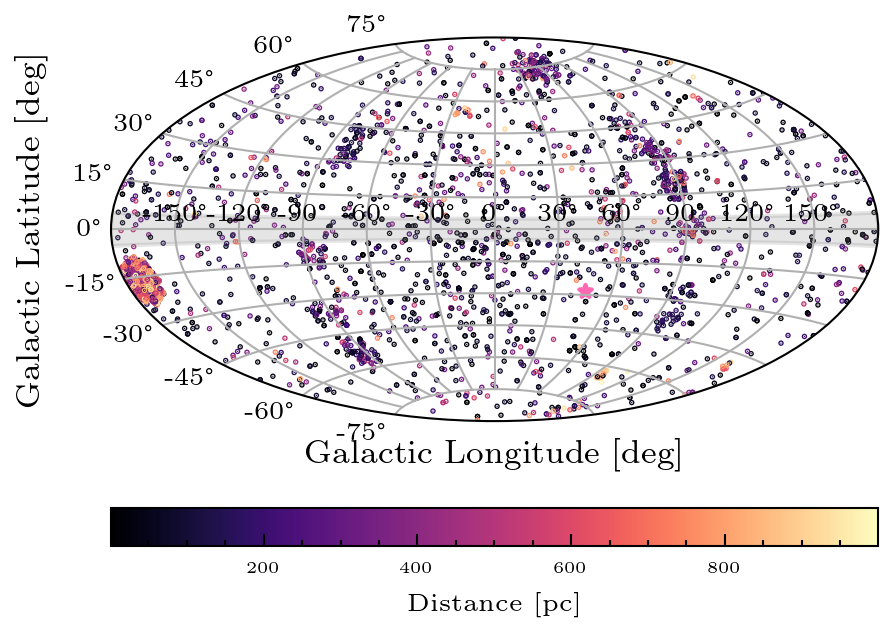
\includegraphics[width=0.6\textwidth]{figures/Science Case Plots/galactic_projection_NEA.png}
    \caption{Some plot here with target of intrests that fall within the zenith pointings and their associated Jy measurements based on Tsys etc. }
    \label{fig:enter-label}
\end{figure}

%PLOTS That could be useful 
% Frequency/Wavelength against Flux Density of Transients -> parameter space plot 
% Variation of Tsys (basically mapping galactic forground) as a function of Lunar Latitude 
% Senstivity as function of integration time 
% Galactic latitude on the x axis, sensitivity on the y, carious longitudes overlapped. 
% Galactic projection plot for areas/exoplanets of intrest, i.e. benchmarking well known targets. 
% Also worth running some numbers to see how much time A team targets are in primary 